\documentclass[12pt]{article}
\usepackage{geometry}
\usepackage{hyperref}
\usepackage{graphicx}
\usepackage{titlesec}
\usepackage{fancyhdr}

% 设置页边距
\geometry{a4paper, left=25mm, right=25mm, top=30mm, bottom=30mm}

% 修复 fancyhdr 警告
\setlength{\headheight}{14.49998pt}

% 页眉页脚设置
\pagestyle{fancy}
\fancyhf{}
\fancyhead[L]{COMP3019J University Website Project}
\fancyhead[R]{\thepage}
\fancyfoot[L]{Group 20}
\fancyfoot[R]{October, 2024}

% 标题格式设置
\titleformat{\section}
  {\large\bfseries}{\thesection}{1em}{}
\titleformat{\subsection}
  {\normalsize\bfseries}{\thesubsection}{1em}{}

% 生成可点击链接
\hypersetup{
    colorlinks=true,
    linkcolor=blue,
    filecolor=magenta,      
    urlcolor=cyan,
    pdftitle={COMP 3019J Project},
    pdfpagemode=FullScreen,
}

% 文档标题
\title{COMP3019J University Website Project\\ \Large Design Document}
\date{October 2024}

\begin{document}

% 第一页:标题页
\maketitle
\vspace{2cm}
\begin{figure}[h]  % 插入图片的部分
  \centering
  
\includegraphics[width=0.5\textwidth]{title.png}  % 替换成你的图片文件名
\end{figure}
\vspace{6cm}

% 插入作者和日期信息作为文本
\begin{center}
  \textbf{Bohan Zhang 22207251}\\
  \textbf{Yunhan Gao 22207250}\\
  \textbf{Le Liu 22207256}\\
\end{center}

\thispagestyle{empty}
\newpage

% 第二页:目录页
\tableofcontents
\newpage

% 开始正文

\section{Introduction}

\subsection{Project Goals}
The primary goal of this project is to design and implement a comprehensive university website that offers a personalized
 and functional experience for different types of users. The website will provide students, teachers, and other university 
 personnel with an interface to manage their profiles, interact with others, and access university resources based on their 
 roles. The website is expected to enhance user engagement, facilitate communication, and streamline administrative processes 
 within the university. Additionally, the project will focus on secure data handling and innovative functionalities to 
 differentiate the website from existing solutions.

\subsection{Target Users and Use Cases} The target users of the website include students, teachers, library staff, security personnel, 
administrative staff and external visitors. Each user type has specific features tailored to their role:

\begin{itemize}
  \item \textbf{Students}: Students will have access to their dashboard, which display timetables, profiles, and
  enrolled courses. They can register for courses, check their grades, interact with teachers and fellow students, view library
  collections, and check their own borrowing history, as well as manage their electric bike licenses.
  \item \textbf{Teachers}: Teachers will have a dashboard that shows the courses they teach, timetable, profiles, and office
  location. They can create and manage courses, interact with students, view library collections.
  \item \textbf{Library staff}: Library staff will have access to features that allow them to manage book inventories, track book
  loans, and assist users with book reservations. They can also update library resources and monitor the availability of digital
  content for users.
  \item \textbf{Security personnel}: Security personnel will manage electric bike licenses and oversee vehicle registrations on
  campus.
  \item \textbf{Administrative staff}: Administrative users will have full control over the system, including managing user
  registrations, overseeing course creation, and handling overall database management to ensure smooth system operation.
  \item \textbf{External visitors}: Unregistered users will have limited access to parts of the website, such as viewing general
  information about the university, available library resources without the ability  interact with internal functions.
\end{itemize}

\subsection{Technological Stack Overview}
The university website will be built using a modern and robust technological stack to ensure reliability, security, and scalability.
The core technologies to be used include:
\begin{itemize}
    \item \textbf{Frontend}: The user interface will be developed using HTML, CSS, and JavaScript to create an interactive and
     responsive design. Libraries like Bootstrap or Material UI may be incorporated for consistent styling across the website.
    \item \textbf{Backend}: The server-side logic will be implemented using Flask (Python), providing a flexible framework for
    managing user authentication, database interactions, and session management.
    \item \textbf{Database}: MySQL will be used as the primary database management system to store user profiles,
    course data, library resources, electric bike licenses, and forum information. The database will include the design of
    tables with appropriate relationships, such as primary and foreign keys, to ensure data integrity and support efficient
    querying and management.
    \item \textbf{Security}: The website will ensure secure handling of sensitive data, such as passwords, using encryption
    mechanisms. Proper user authentication and authorization will be implemented to protect user privacy and data access.
\end{itemize}
This technology stack has been chosen for its simplicity, flexibility, and suitability for the scale of the university website project,
ensuring a smooth user experience and maintainability.

\newpage
\section{Website Functionalities}
\subsection{User Registration and Account Management}
% 在这里详细描述用户注册和账号管理功能。
\subsection{User Types and Role-Specific Features}
% 在这里描述不同类型用户及其特定功能。
\subsection{Profile Customization and Display}
% 在这里描述用户个人资料定制和展示功能。
\subsection{User Interaction and Communication}
% 在这里描述用户之间的交互和沟通方式。
\subsection{Unregistered User Access}
% 在这里描述未注册用户的有限访问权限。
\subsection{Security and Data Protection}
% 在这里详细描述安全性和数据保护措施。
\subsection{Administrative Features}
% 在这里描述管理员账户和其功能。
\subsection{Extra Functionality}
% 在这里描述额外的功能。

\newpage
\section{Database Design}

\subsection{Entity-Relationship Diagrams}
The database for the university website currently includes several key tables: \texttt{user},
\texttt{student\_profile}, \texttt{teacher\_profile}, \texttt{library\_staff\_profile},
\texttt{security\_personnel\_profile}, \texttt{course}, \texttt{course\_registration}, \texttt{library\_resources},
\texttt{library\_loan}, \texttt{e\_bike\_license}, \texttt{forum\_post} and \texttt{forum\_reply}.\\ \\
These tables represent the foundational structure for managing users and their interactions with the system,
such as course enrollment and profile management. To support additional functionalities outlined in the introduction,
tables have been added to manage library resources, electric bike licenses, and forum discussions.
These expansions ensure that students, teachers, library staff, and security personnel can effectively interact
with the system in their respective roles. \\ \\
The Entity-Relationship Diagrams are on the next page:

\begin{figure}[htbp]
  \centering
  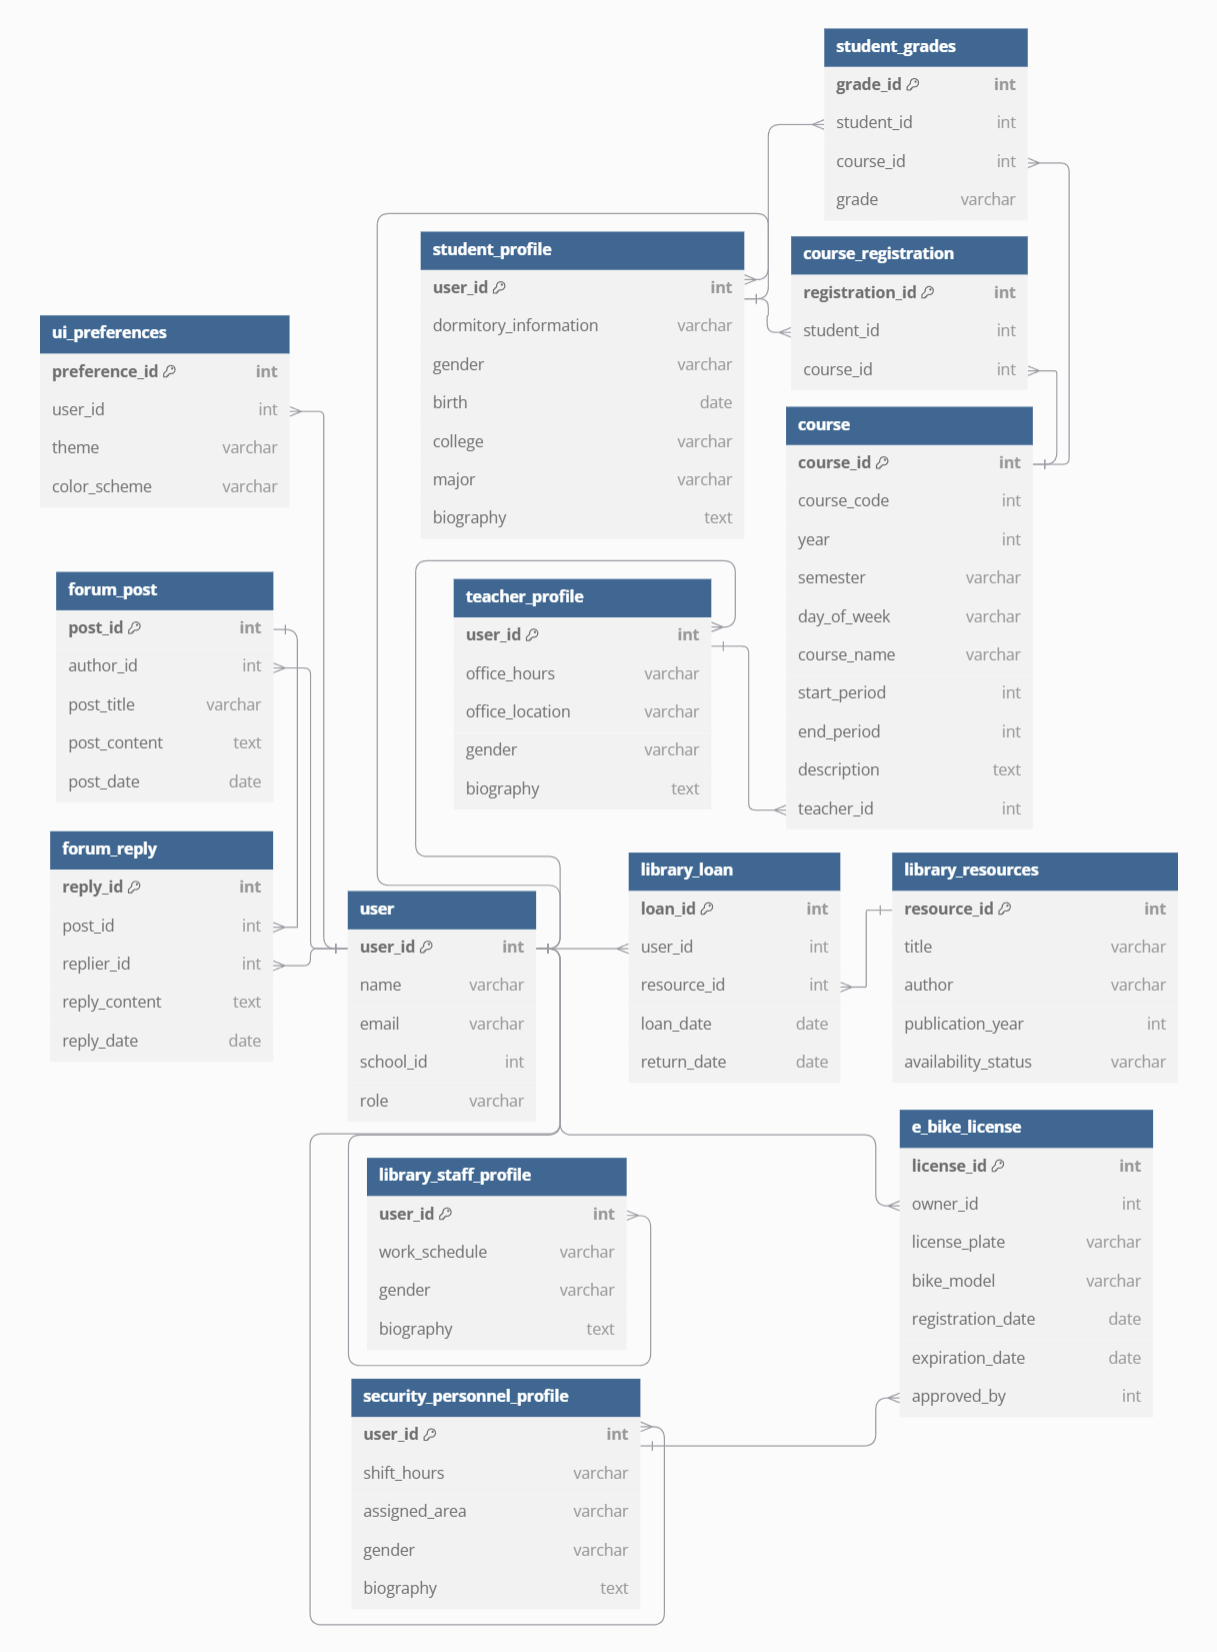
\includegraphics[width=\textwidth, height=0.8\textheight, keepaspectratio]{ER.png}
  \caption{Entity-Relationship Diagram}
\end{figure}

\clearpage  % 强制换页,并将后续内容移到图片的下一页

\subsection{Table Structures and Relationships}
Below are the current and proposed tables, along with their respective fields and relationships:

\begin{itemize}
    \item \texttt{user}: Contains user information common to all user types. Fields include:
    \begin{itemize}
        \item \texttt{user\_id} (Primary Key)
        \item \texttt{name}
        \item \texttt{email}
        \item \texttt{school\_id}
        \item \texttt{role} (e.g., student, teacher, library staff, security personnel)
    \end{itemize}

    \item \texttt{student\_profile}: Stores additional information specific to students. Fields include:
    \begin{itemize}
        \item \texttt{user\_id} (Foreign Key referencing \texttt{user})
        \item \texttt{dormitory\_information}
        \item \texttt{gender}
        \item \texttt{birth}
        \item \texttt{college}
        \item \texttt{major}
        \item \texttt{biography}
    \end{itemize}

    \item \texttt{teacher\_profile}: Stores additional information specific to teachers. Fields include:
    \begin{itemize}
        \item \texttt{user\_id} (Foreign Key referencing \texttt{user})
        \item \texttt{office\_hours}
        \item \texttt{office\_location}
        \item \texttt{gender}
        \item \texttt{biography}
    \end{itemize}

    \item \texttt{library\_staff\_profile}: Stores additional information specific to library staff. Fields include:
    \begin{itemize}
        \item \texttt{user\_id} (Foreign Key referencing \texttt{user})
        \item \texttt{work\_schedule}
        \item \texttt{gender}
        \item \texttt{biography}
    \end{itemize}

    \clearpage  % 强制换页,并将后续内容移到图片的下一页

    \item \texttt{security\_personnel\_profile}: Stores additional information specific to security personnel. Fields include:
    \begin{itemize}
        \item \texttt{user\_id} (Foreign Key referencing \texttt{user})
        \item \texttt{shift\_hours}
        \item \texttt{assigned\_area}
        \item \texttt{gender}
        \item \texttt{biography}
    \end{itemize}


    \item \texttt{course}: Contains information about the courses offered. Fields include:
    \begin{itemize}
        \item \texttt{course\_id} (Primary Key)
        \item \texttt{course\_code}
        \item \texttt{year}
        \item \texttt{semester}
        \item \texttt{day\_of\_week}
        \item \texttt{course\_name}
        \item \texttt{start\_period}
        \item \texttt{end\_period}
        \item \texttt{description}
        \item \texttt{teacher\_id} (Foreign Key referencing \texttt{teacher\_profile})
    \end{itemize}

    \item \texttt{course\_registration}: Tracks student registrations for courses. Fields include:
    \begin{itemize}
        \item \texttt{registration\_id} (Primary Key)
        \item \texttt{student\_id} (Foreign Key referencing \texttt{student\_profile})
        \item \texttt{course\_id} (Foreign Key referencing \texttt{course})
    \end{itemize}

    \item \texttt{student\_grades}: Stores student's grade for each course. Fields include:
    \begin{itemize}
        \item \texttt{grade\_id} (Primary Key)
        \item \texttt{student\_id} (Foreign Key referencing \texttt{student\_profile})
        \item \texttt{course\_id} (Foreign Key referencing \texttt{course})
        \item \texttt{grade} (The grade received by the student)
    \end{itemize}

    % 新增的表格
    \item \texttt{library\_resources}: Manages library books and resources. Fields include:
    \begin{itemize}
        \item \texttt{resource\_id} (Primary Key)
        \item \texttt{title}
        \item \texttt{author}
        \item \texttt{publication\_year}
        \item \texttt{availability\_status}
    \end{itemize}

    \item \texttt{library\_loan}: Tracks book loans by students and other users. Fields include:
    \begin{itemize}
        \item \texttt{loan\_id} (Primary Key)
        \item \texttt{user\_id} (Foreign Key referencing \texttt{user})
        \item \texttt{resource\_id} (Foreign Key referencing \texttt{library\_resources})
        \item \texttt{loan\_date}
        \item \texttt{return\_date}
    \end{itemize}

    \item \texttt{e\_bike\_license}: Manages electric bike licenses for students, teachers, and library staff. Fields include:
    \begin{itemize}
        \item \texttt{license\_id} (Primary Key)
        \item \texttt{owner\_id} (Foreign Key referencing \texttt{user})
        \item \texttt{license\_plate}
        \item \texttt{bike\_model}
        \item \texttt{registration\_date}
        \item \texttt{expiration\_date}
        \item \texttt{approved\_by} (Foreign Key referencing \texttt{security\_personnel\_profile})
    \end{itemize}

    \item \texttt{forum\_post}: Stores user-created posts for the forum. Fields include:
    \begin{itemize}
        \item \texttt{post\_id} (Primary Key)
        \item \texttt{author\_id} (Foreign Key referencing \texttt{user})
        \item \texttt{post\_title}
        \item \texttt{post\_content}
        \item \texttt{post\_date}
    \end{itemize}

    \item \texttt{forum\_reply}: Stores user replies to forum posts. Fields include:
    \begin{itemize}
        \item \texttt{reply\_id} (Primary Key)
        \item \texttt{post\_id} (Foreign Key referencing \texttt{forum\_post})
        \item \texttt{replier\_id} (Foreign Key referencing \texttt{user})
        \item \texttt{reply\_content}
        \item \texttt{reply\_date}
    \end{itemize}

    \item \texttt{ui\_preferences}: Stores user preferences for the UI interface. Fields include:
    \begin{itemize}
        \item \texttt{preference\_id} (Primary Key)
        \item \texttt{user\_id} (Foreign Key referencing \texttt{user})
        \item \texttt{theme} (Preferred UI theme, e.g., light, dark)
        \item \texttt{color\_scheme} (Preferred color scheme, e.g., blue, green)
    \end{itemize}
\end{itemize}

\subsection{Primary and Foreign Key Design}
Each table contains a primary key that uniquely identifies each record. Foreign keys are used to establish relationships between users and the entities they interact with. For example:
\begin{itemize}
    \item The \texttt{user\_id} field in \texttt{student\_profile}, \texttt{teacher\_profile},
    \texttt{library\_staff\_profile}, and \texttt{security\_personnel\_profile} links the
    profiles to the core \texttt{user} table.
    \item The \texttt{course\_id} field in \texttt{course\_registration} and \texttt{student\_grades} links
    students to the courses they have enrolled in and the grades they have received.
    \item The \texttt{license\_id} in the \texttt{e\_bike\_license} table allows students
    to register electric bikes, which are approved by security personnel.
    \item The \texttt{post\_id} and \texttt{reply\_id} in the \texttt{forum\_post} and \texttt{forum\_reply}
    tables link forum posts and their replies to the users who created them.
    \item The \texttt{user\_id} field in the \texttt{ui\_preferences} table links users to their personalized
    interface settings, such as theme, font size, and color scheme.
\end{itemize}

\subsection{Data Population Strategy}
The initial data for the \texttt{user}, \texttt{course}, and \texttt{library\_resources}
tables will be seeded by administrators during development and testing phases. As users
interact with the system, data will be dynamically added to the \texttt{course\_registration},
\texttt{student\_grades}, \texttt{library\_loan}, \texttt{e\_bike\_license}, \texttt{forum\_post},
\texttt{forum\_reply}, and \texttt{ui\_preferences} tables. The system will ensure that all data
remains up-to-date and consistent across these entities, allowing users to track their course
registrations, grades, library loans, and personalized interface preferences.

\newpage
\section{Web Page Design}
\subsection{Mockups and Layout Overview}
% 在这里插入网页设计草图并描述布局。
% \begin{figure}[h]
%     \centering
%     \includegraphics[width=0.8\textwidth]{path_to_your_mockup.png}
%     \caption{Web Page Mockup}
% \end{figure}
\subsection{Color Schemes and Style Guidelines}
% 在这里描述网页的配色方案和风格指南。
\subsection{User Experience Considerations}
% 在这里描述用户体验相关的设计考量。
\subsection{Responsive Design}
% 在这里描述响应式设计方案。

\newpage
\section{Technical Details}
\subsection{File and Directory Structure}
% 在这里描述项目的文件和目录结构。
\subsection{Code Components and Dependencies}
% 在这里描述代码的各个组成部分和依赖关系。
\subsection{API and Database Interaction}
% 在这里描述API与数据库的交互方式。
\subsection{Version Control and Repository Details}
% 在这里描述版本控制系统的使用和代码库的详细信息。

\newpage
\section{Conclusion}
\subsection{Summary of Features}
% 在这里总结网站功能。
\subsection{Future Development Plans}
% 在这里描述未来的开发计划和功能改进。

\end{document}